\section{Delta}\label{Demo}

\begin{figure*}[t]
  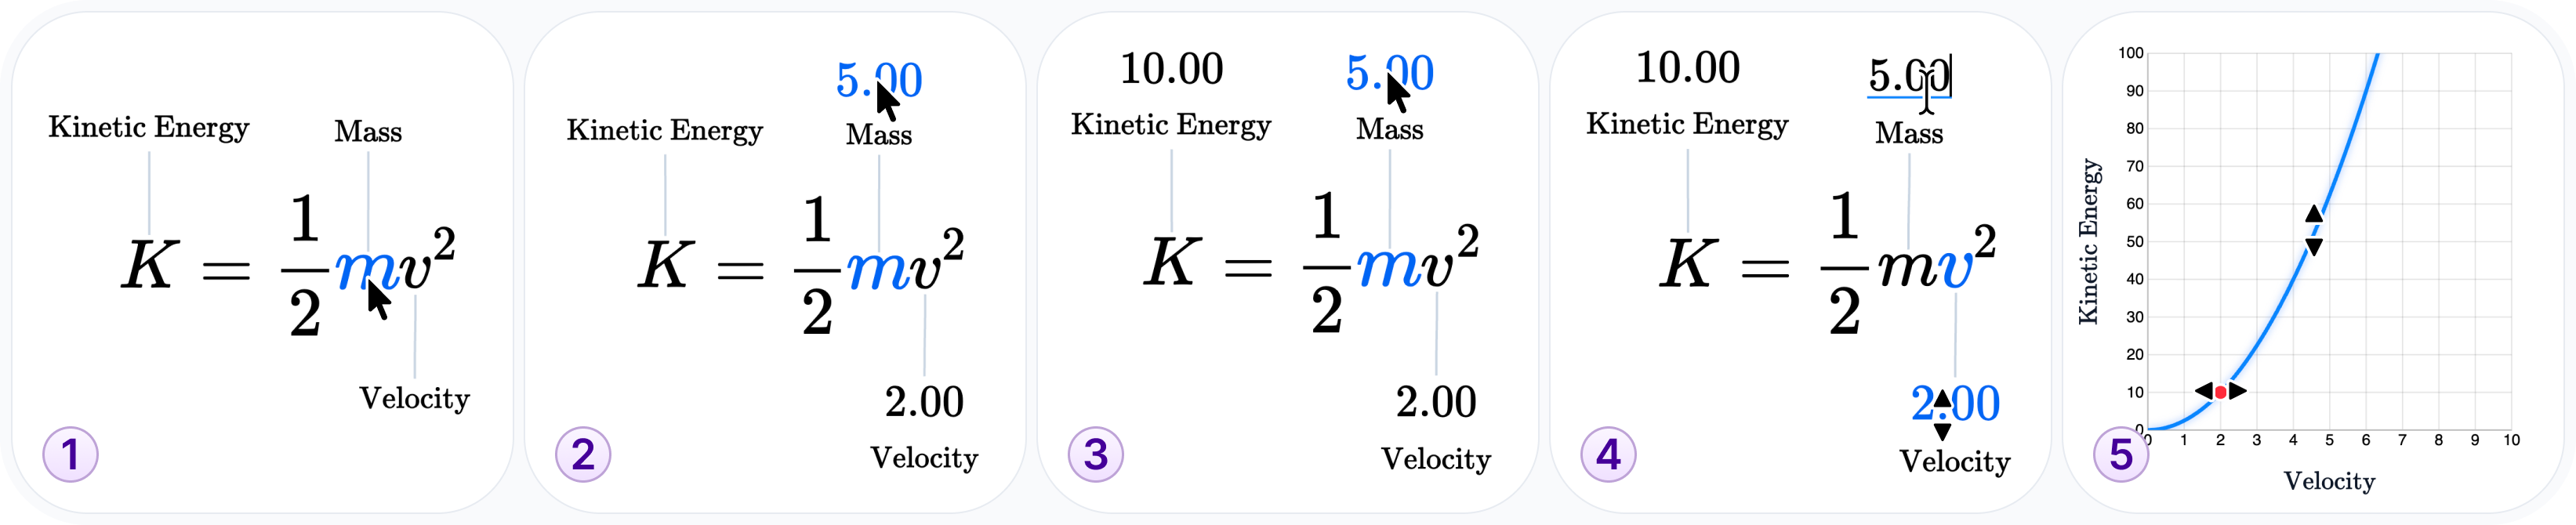
\includegraphics[width=\textwidth]{fig/demo-1.png}
  \caption{Outputs from creating a simple calculator. \textmd{(1) Adding labels. (2) Showing default values for exploration. (3) Computing derived variables live. (4) Input modes (variable dragging and inline editing). (5) Bidirectional connections with interactive plot.}}
  \label{fig:demo-1}
\end{figure*}

Delta is designed to provide a low threshold and high ceiling for adding interactivity to formulas in web documents. We illustrate the low threshold with a walkthrough of creating the simplest augmentations in Section~\ref{Basics}, describe the full set of constructs and their design philosophy Section~\ref{Language}, and hint at the high ceiling by reviewing a gallery of examples we created with Delta in Section~\ref{Gallery}.

\subsection{Basics}\label{Basics}

To author interactive formulas in Delta, an author writes a \texttt{Config}, an object that holds the main constructs of the language. An author defines \emph{formulas} in typical LaTeX, selects and attaches interaction properties to \emph{variables}, and attaches \emph{semantics} via a JavaScript function. Optionally, they provide \emph{connections} to other visuals and break down explanations into \emph{steps}. We introduce each construct as it arises in example tasks below.

\subsubsection{Simple calculation}
Imagine an author making an interactive calculator from the physics formula, $K = \frac{1}{2}mv^2$. Their intent is to label the major variables, let readers play with different values of mass ($m$) and velocity ($v$) to see how kinetic energy ($K$) changes, and clarify the relationships in a graph (end goal in Figure~\ref{fig:demo-1}). The author first defines the base \textbf{\emph{formula}} in standard LaTeX:

\begin{tcolorbox}[codebox]
\begin{lstlisting}[style=jsstyle]
const kineticConfig: Config = {
  formulas: [
    id: "kinetic-energy", latex: "K = \\frac{1}{2}mv^2",
  ]
}
\end{lstlisting}
\end{tcolorbox}

Macro commands are escaped (``\texttt{\textbackslash{}\textbackslash{}}'') since they appear in a JavaScript string. The `id' serves as a handle for inserting this formula into a Delta React component, and \texttt{Config} houses all specification of the formula's behavior. Next, the author sketches out the basics of interaction by selecting key \textbf{\emph{variables}} with descriptive labels (Figure~\ref{fig:demo-1}.1) and recommended default values:

\begin{tcolorbox}[codebox]
\begin{lstlisting}[style=jsstyle]
const kineticConfig: Config = { ...
  variables: {
    K: { name: "Kinetic Energy" },
    m: { name: "Mass", default: 5 },
    v: { name: "Velocity", default: 2 },
  },
}
\end{lstlisting}
\end{tcolorbox}

To refer to a variable, the author writes its literal form from the original LaTeX. Variables can be multi-letter expressions; here they are just individual letters. To use the formula in a React document, the author wraps their content in a \textbf{\emph{provider}} component that accepts the configuration: \verb|<Provider config={kineticConfig}>|. Placing \verb|<Formula id="kinetic-energy"/>| inside the provider produces a typeset formula with descriptive labels in the margins and starter values for experimentation. Labels are visually linked to expressions; hovering over values highlights the corresponding term in the formula (Figure~\ref{fig:demo-1}.2). 

To turn the formula into a calculator, the author defines the \textbf{\emph{semantics}} of the formula. The semantics is a JavaScript function that serves three roles: it \emph{computes} derived variable values from inputs, it can \emph{sample} data points to populate linked graphs, and it can insert \emph{steps} that annotate the formula with labels and descriptions for guided walkthroughs. We start with the simplest use---computation:

\begin{tcolorbox}[codebox]
\begin{lstlisting}[style=jsstyle]
semantics: function ({ vars }) {
   vars.K = 0.5 * vars.m * Math.pow(vars.v, 2);
},
\end{lstlisting}
\end{tcolorbox}

This is a standard JavaScript function doing math. The semantics function maps input variables to outputs: the author reads from a \texttt{vars} object and writes to output variables---here, reading \texttt{m} and \texttt{v} to compute \texttt{K}. Variable keys match those defined in the \texttt{variables} spec. The formula is now interactive (Figure~\ref{fig:demo-1}.3): a reader can click and drag on $m$ and $v$ to change values and see $K$ update live. The author can further configure interaction with a few simple properties---here, allowing free-text input for mass and constraining ranges to sensible values (e.g., no negative masses) (Figure~\ref{fig:demo-1}.4):

\begin{tcolorbox}[codebox]
\begin{lstlisting}[style=jsstyle]
m: { name: "Mass", default: 5, 
     input: "inline", range: [0, 20] },
v: { name: "Velocity", default: 2,
     input: "drag", range: [0, 10] },
\end{lstlisting}
\end{tcolorbox}

\subsubsection{Linked visual}
The author can add \textbf{\textit{connections}} between formulas and other representations elsewhere in the document. Delta provides a dedicated construct interactive 2D and 3D plots. To create a plot where a user can tinker with values and curves in tandem with the formula, the author adds a graph:

\begin{tcolorbox}[codebox]
\begin{lstlisting}[style=jsstyle]
graph2d: [{
  id: "energy-graph",
  xAxisVar: "v", yAxisVar: "K",
  lines: [{
    sampleId: "energy", parameter: "v",
    interaction: ["vertical-drag", "m"],
  }],
  points: [{
    sampleId: "energy",
    interaction: ["horizontal-drag", "v"],
  }],
}],
\end{lstlisting}
\end{tcolorbox}

This creates a 2D graph, associates axes with specific variables (\texttt{xAxisVar} with \texttt{v}, \texttt{yAxisVar} with \texttt{K}), and specifies the source of curve points (a sample called \texttt{energy}). Points come from samples collected in the semantics function, where \texttt{sample} records a named set of data points each time the semantics is evaluated over a range of input values:

\begin{tcolorbox}[codebox]
\begin{lstlisting}[style=jsstyle]
semantics: function ({ vars, sample }) {
  vars.K = 0.5 * vars.m * Math.pow(vars.v, 2);
  sample("energy", { x: vars.v, y: vars.K });
},
\end{lstlisting}
\end{tcolorbox}

Optional \texttt{interaction} fields allow manipulation on the plot to map back to the formula: vertical drags change the curve by altering \texttt{m}, and horizontal drags move \texttt{v} along the curve. Interaction is bidirectional---tinkering with formula labels updates the curve and point position, and vice versa. The graph is rendered with a React \texttt{Graph} component referencing the graph ID. Connections to arbitrary custom content are possible through mechanisms described in Section~\ref{Language}.

\paragraph{Simple walkthrough}\label{Average}

An author may want to guide attention to different parts of a formula one piece at a time. A special case involves formulas describable through incremental calculations---for instance, the average $\mu = \frac{1}{n} \sum_{i=1}^{n} X_i$ could be shown as incrementally adding summands then dividing by $n$. For such cases, Delta lets authors provide explanations as series of \textbf{\emph{steps}} inserted into the semantics, since the JavaScript function already supports sequence and iteration, and sequence sometimes benefits from alignment with simulated calculation. For instance, in this part of the average computation (sum shown):

\begin{figure}[t]
  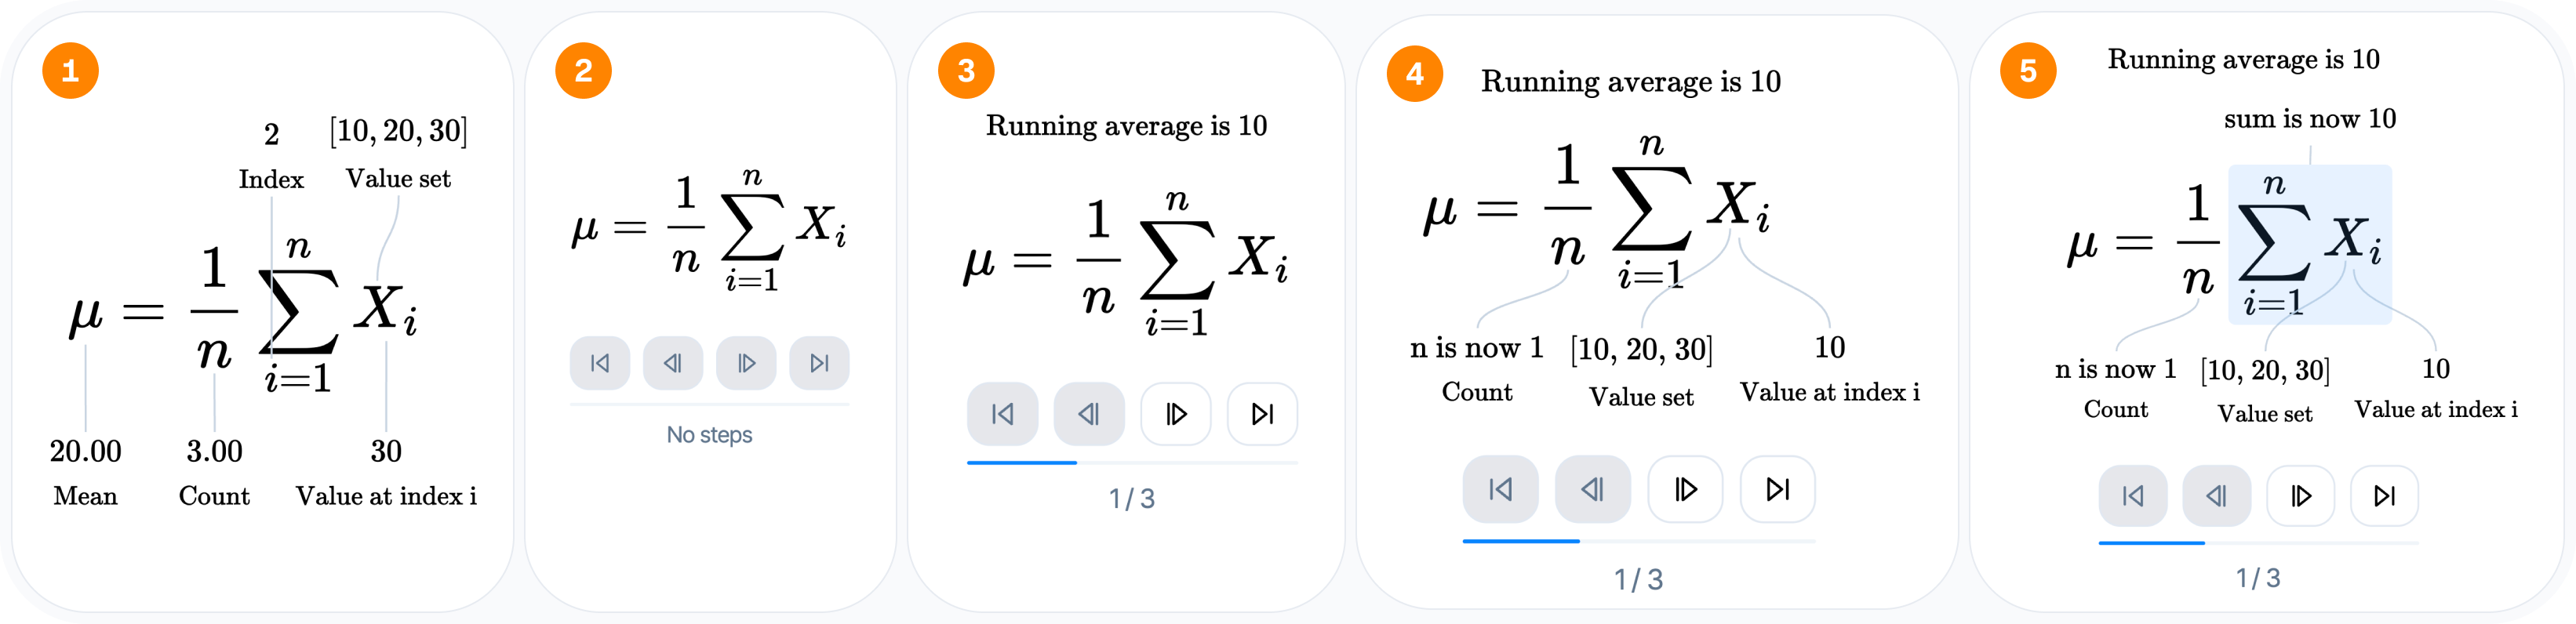
\includegraphics[width=\columnwidth]{fig/demo-2.png}
  \caption{A step in the average formula walkthrough. LaTeX keys (e.g., \texttt{"X\_i"}) serve as selectors to anchor labels onto corresponding notation spans.}
  \label{fig:demo-2}
\end{figure}

\begin{tcolorbox}[codebox]
\begin{lstlisting}[style=jsstyle]
semantics: function ({ vars }) { ...
  // [elided] define n, sum, initial \\mu value
  for (var i = 0; i < vars.n; i++) {
    vars.i = i;
    vars.X_i = vars.X[i];
    sum += vars.X_i;
    vars["\\mu"] = sum / (i + 1); // approximate running average
  } ...
},
\end{lstlisting}
\end{tcolorbox}

The author would add this step:

\begin{tcolorbox}[codebox]
\begin{lstlisting}[style=jsstyle]
for (var i = 0; i < vars.n; i++) {
  // ...
  step({
    description: "Running average is " + vars["\\mu"],
    labels: {
      "\\sum_{i=1}^{n} X_i": "sum is now " + sum,
      n: "n is now " + (i + 1),
      X_i: vars.X_i,
      X: vars.X,
    },
  });
}
\end{lstlisting}
\end{tcolorbox}

This produces labels shown at each stage of the walkthrough, which can be navigated forward and back. Labels can include calculated values (Figure~\ref{fig:demo-2}). An arbitrary number of steps can be added; they appear in walkthrough order matching the order encountered during semantics execution.